\documentclass[a4paper]{article}
\usepackage[utf8]{vietnam}
\usepackage{graphics}
\usepackage{float}
\usepackage{a4wide,amssymb,epsfig,latexsym,array,hhline,fancyhdr}
\usepackage[normalem]{ulem}
\usepackage[makeroom]{cancel}
\usepackage{amsmath}
\usepackage{amsthm}
\usepackage{multicol,longtable,amscd}
\usepackage{diagbox}%Make diagonal lines in tables
\usepackage{booktabs}
\usepackage{alltt}
\usepackage[framemethod=tikz]{mdframed}% For highlighting paragraph backgrounds
\usepackage{caption,subcaption}

\usepackage{lastpage}
\usepackage[lined,boxed,commentsnumbered]{algorithm2e}
\usepackage{enumerate}
\usepackage{color}
\usepackage{graphicx}							% Standard graphics package
\usepackage{array}
\usepackage{tabularx, caption}
\usepackage{multirow}
\usepackage{multicol}
\usepackage{rotating}
\usepackage{graphics}
\usepackage{geometry}
\usepackage{setspace}
\usepackage{epsfig}
\usepackage{tikz}
\usetikzlibrary{arrows,snakes,backgrounds}
\usepackage[unicode]{hyperref}
\hypersetup{urlcolor=blue,linkcolor=black,citecolor=black,colorlinks=true} 


\usepackage[normalem]{ulem}

\newtheorem{theorem}{{\bf Định lý}}
\newtheorem{property}{{\bf Tính chất}}
\newtheorem{proposition}{{\bf Mệnh đề}}
\newtheorem{corollary}[proposition]{{\bf Hệ quả}}
\newtheorem{lemma}[proposition]{{\bf Bổ đề}}
\theoremstyle{definition}
\newtheorem{exer}{Bài toán}

\def\thesislayout{	% A4: 210 × 297
	\geometry{
		a4paper,
		total={160mm,240mm},  % fix over page
		left=30mm,
		top=30mm,
	}
}
\thesislayout


\setlength{\headheight}{40pt}
\pagestyle{fancy}
\fancyhead{} % clear all header fields
\fancyhead[L]{
	\begin{tabular}{rl}
		\begin{picture}(25,15)(0,0)
			\put(0,-8){
\includegraphics[width=8mm, height=8mm]{Images/hcmut.png}}
			%\put(0,-8){\epsfig{width=10mm,figure=hcmut.eps}}
		\end{picture}&
		%
\includegraphics[width=8mm, height=8mm]{hcmut.png} & %
		\begin{tabular}{l}
			\textbf{\bf \ttfamily Trường Đại Học Bách Khoa Tp.Hồ Chí Minh}\\
			\textbf{\bf \ttfamily Khoa Khoa Học \& Kỹ Thuật Máy Tính}
		\end{tabular} 	
	\end{tabular}
}
\fancyhead[R]{
	\begin{tabular}{l}
		\tiny \bf \\
		\tiny \bf 
\end{tabular}  }
\fancyfoot{} % clear all footer fields
\fancyfoot[L]{\scriptsize \ttfamily Đề bài tập lớn môn Cấu trúc Rời rạc cho KHMT (CO1007) - Niên khóa 2021-2022}
\fancyfoot[R]{\scriptsize \ttfamily Trang {\thepage}/\pageref{LastPage}}
\renewcommand{\headrulewidth}{0.3pt}
\renewcommand{\footrulewidth}{0.3pt}


%%%
\setcounter{secnumdepth}{4}
\setcounter{tocdepth}{3}
\makeatletter
\newcounter {subsubsubsection}[subsubsection]
\renewcommand\thesubsubsubsection{\thesubsubsection .\@alph\c@subsubsubsection}
\newcommand\subsubsubsection{\@startsection{subsubsubsection}{4}{\z@}%
	{-3.25ex\@plus -1ex \@minus -.2ex}%
	{1.5ex \@plus .2ex}%
	{\normalfont\normalsize\bfseries}}
\newcommand*\l@subsubsubsection{\@dottedtocline{3}{10.0em}{4.1em}}
\newcommand*{\subsubsubsectionmark}[1]{}
\makeatother

\everymath{\color{blue}}%make in-line maths symbols blue to read/check easily

\sloppy
\captionsetup[figure]{labelfont={small,bf},textfont={small,it},belowskip=-1pt,aboveskip=-9pt}

\captionsetup[table]{labelfont={small,bf},textfont={small,it},belowskip=-1pt,aboveskip=7pt}

\setlength{\floatsep}{5pt plus 2pt minus 2pt}
\setlength{\textfloatsep}{5pt plus 2pt minus 2pt}
\setlength{\intextsep}{10pt plus 2pt minus 2pt}

\thesislayout

\begin{document}
	\begin{titlepage}
		\begin{center}
			ĐẠI HỌC QUỐC GIA THÀNH PHỐ HỒ CHÍ MINH \\
			TRƯỜNG ĐẠI HỌC BÁCH KHOA \\
			KHOA KHOA HỌC \& KỸ THUẬT MÁY TÍNH
		\end{center}
		\vspace{1cm}
		\begin{figure}[h]
			\centering
			
\includegraphics[width=3cm]{images/hcmut.png}
		\end{figure}	
		\begin{center}
			\begin{tabular}{c}
				\multicolumn{1}{l}{\textbf{{\Large CẤU TRÚC RỜI RẠC CHO KHMT (CO1007)}}}\\
				~~\\
				\hline
				\\
				\textbf{\large Thống kê khảo sát kết quả Covid-19}\\
				\textbf{\large môn Cấu trúc rời rạc}
				\\
				\hline
			\end{tabular}
		\end{center}
		\begin{table}[h]
			\centering
			\begin{tabular}{rrl}
				\hspace{2 cm} & GVHD: & Huỳnh Tường Nguyên\\
				\hspace{2 cm} &  & Nguyễn Ngọc Lễ\\
				
				& SV thực hiện: & Lê Văn Tuấn Kiệt -- 2110300 \\
				& & Dương Ngọc Ân -- 2110030 \\
				& & Phan Lê Nhật Minh -- 2114066 \\
				& & Cù Hoàng Nguyễn Sơn -- 2112185 \\
				& & Từ Huy Bảo -- 2112887 \\
				& & Nguyễn Hồng Quân -- 2112122 \\
			\end{tabular}
		\end{table}
		\vspace{1.5cm}
		\begin{center}
			{\footnotesize Tp. Hồ Chí Minh, Tháng 03/2022}
		\end{center}
	\end{titlepage}
	\newpage
	\tableofcontents
	\newpage
	\section{Động cơ nghiên cứu}\label{motivation}
	$\indent$Bệnh Corona do virus gây ra còn gọi là COVID-19 đã tạo ra những tác động tiêu cực đến nền đời sống của cư dân trên thề giới. Các đợt bùng phát của COVID-19 hay những biến thể virus đã mang đến những thách thức chưa từng có và được dự báo sẽ có tác động đáng kể đến sự phát triển kinh tế. Nhiều thông tin, tin tức về tình hình dịch bệnh cũng như dữ liệu về COVID-19 được phổ biến rộng rải trong đời sống hay trên internet để giúp cho mọi người quan sát, phân tích, nghiên cứu đươc cập nhật hàng ngày.
	
	Phân tích \& thống kê dữ liệu về COVID-19 giúp cho ta thấy được số ca nhiễm bệnh, tử vong của một quốc gia, so sánh tình trạng của các quốc gia trong khu vực hay diễn biến dịch trên thế giới. Từ số liệu được báo cáo mơi chúng ta muốn biết các ca nhiễm bệnh có xu hướng tăng lên hay giảm xuống quy mô các đợt bùng phát ở mỗi quốc gia. Dữ liệu dùng cho bài tập lớn có tham khào từ \hyperlink{https://github.com/owid/covid-19-data/blob/master/public/data/README.md}{nguồn} có thể xử lý trước với một vài thống kê cơ bản trước khi nó được truyền đi để khai thác dữ liệu thông minh sâu hơn.
	\section{Mục tiêu}\label{objective}
	$\indent$  
	Trong bài tập lớn này, chúng ta sẽ bắt đầu với các bài toán thống kê đơn giản từ những dữ liệu được cung cấp. Qua đó, ta tìm ra những con số thú vị, có ý nghĩa đối với các dữ liệu thực tế từ tình hình dịch corona. Những kết quả mà tìm ra sẽ là bước khởi đầu cho việc khai phá nguồn dữ liệu của hệ thống sau này, nhằm đạt tới mục tiêu nâng cao kỹ năng lập trình, kỹ năng giải quyết vấn đề cho người học, kỹ năng làm việc nhóm cũng như hướng tới mục tiêu cao hơn là đam mê trong làm việc, học tập và nghiên cứu
	\section{Mô tả dữ liệu}\label{sec:dataset}
	
	$\indent$Dữ liệu gồm các thuộc tính chính  {\bf ``iso\_code, continent, location, date, new\_cases,	new\_deaths''} được lưu tron file \textbf{csv}. 
	\begin{enumerate}
		\item $iso\_code$: Định danh đất nước 
		\item $continent$ Tên châu lục
		\item $location$: Tên quốc gia
		\item $date$: Ngày quan sát với định dạng Month-Day-Year
		\item $new\_cases$: Số trường hợp COVID-19 mới được xác nhận 
		\item $new\_deaths$: Số tử vong mới do COVID-19 
	\end{enumerate}
	\section{Nhiệm vụ}\label{requirement} 
	\begin{enumerate}[i)]
		\item \textcolor{orange}{Nhóm câu hỏi liên quan đến tổng quát dữ liệu}\\
	Giai đoạn trước đó:\\
	    \begin{itemize}
    \item Lưu bảng dữ liệu thô vào biến bigTable\\
    \item Lưu bảng dữ liệu sau khi lọc bớt các hàng không có châu lục vào biến tableNoNull\\
    \item Lưu các biến này vào preTask.RData bằng câu lệnh save.image("workspace/preTask.RData") để có thể tái sử dụng.\\
        \end{itemize}
    Cài đặt một số packages: readr, ggplot2, stringr, dplyr.\\
    \\
    Một số hàm quan trọng được dùng trong bài i:\\
        \begin{itemize}
    \item Hàm str\_sub để trích xuất các phần tử cuối của một chuỗi ký tự.\\
    \item Hàm unique để lọc các dữ liệu trùng nhau\\
    \item Hàm write và write.csv để ghi file\\
    \item Hàm subset để trích xuất một bảng dữ liệu con với một điều kiện nào đó\\
    \item Hàm append để thêm một phần tử vào một vector\\
    \item Hàm tail và head trả về một số phần tử cuối cùng, hoặc phần tử đầu tiên của vector, list, khung dữ liệu,...\\
    \item Hàm length lấy hoặc ghi độ dài của vector\\
    \item Hàm data.frame để nhập hai khung dữ liệu lại thành một\\
        \end{itemize}
    Cuối cùng, lưu lại các biến để có thể tái sử dụng bằng save.image
			\begin{enumerate}[1)]
				\item Tập mẫu thể hiện thu thập dữ liệu vào các năm:\\
				\\
				2020, 2021 và 2022
				\\
				\item Số lượng đất nước và định danh của mỗi đất nước:
				\begin{figure}[H]
					\centering
					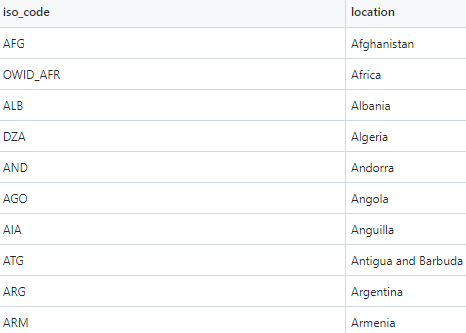
\includegraphics{images/1.2.png}
				\end{figure}
				\item Số lượng đất nước: 238
				\\
				\item Số lượng châu lục trong tập mẫu
					\begin{figure}[H]
						\centering
						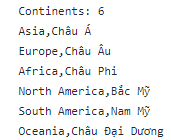
\includegraphics{images/1.3.png}
					\end{figure}
			\item Số lượng dữ liệu thể hiện thu thập dữ liệu được trong từng từng châu lục và tổng số
			\begin{figure}[H]
				\centering
				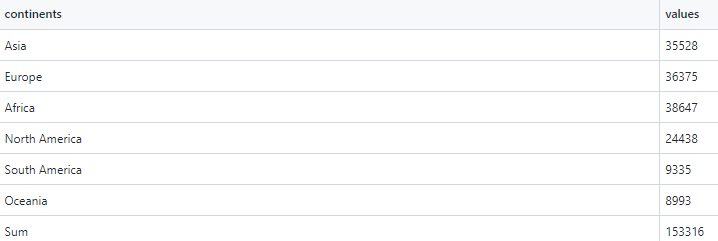
\includegraphics[scale=0.8]{images/1.4.png}
			\end{figure}
			\item Số lượng dữ liệu thể hiện thu thập dữ liệu được trong từng từng đất nước (hiển thị 10 dất nước cuối cùng) và tổng s
			\begin{figure}[H]
				\centering
				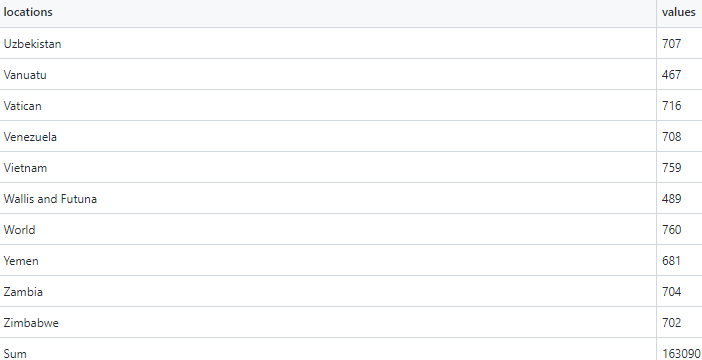
\includegraphics[scale=0.8]{images/1.5.png}
			\end{figure}
			\item Cho biết các châu lục nào có lượng dữ liệu thu thập nhỏ nhất và giá trị nhỏ nhất đó?\\
			\\
			$\indent$
			Châu lục có lượng dữ liệu thu thập nhỏ nhất là Châu Đại Dương với giá trị là 8993\\
			\\
			\item Cho biết các châu lục nào có lượng dữ liệu thu thập lớn nhất và giá trị lớn nhất đó?\\
			\\
			$\indent$
			Châu lục có lượng dữ liệu thu thập lớn nhất là Châu Phi với giá trị là 38647 \\
			\\
			\item Cho biết các nước nào có lượng dữ liệu thu thập nhỏ nhất và giá trị nhỏ nhất đó?\\
			\\
			$\indent$
			Nước có ít dữ liệu thu thập nhỏ nhất là Pitcairn với giá trị là 85\\
			\\
			\item Cho biết các nước nào có lượng dữ liệu thu thập lớn nhất và giá trị lớn nhất đó?\\
			\\
			$\indent$
			Nước có ít dữ liệu thu thập lớn nhất là Argentina và Mexico với giá trị là 781\\
			\\
			\item Cho biết các date nào có lượng dữ liệu thu thập nhỏ nhất và giá trị nhỏ nhất đó?\\
			\\
			$\indent$
			\begin{figure}[H]
				\centering
				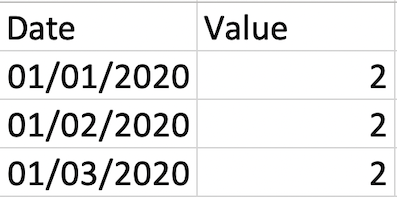
\includegraphics{images/1.10.png}
			\end{figure}
			\item Cho biết các date nào có lượng dữ liệu thu thập lớn nhất và giá trị lớn nhất đó?\\
			$\indent$
			\begin{figure}[H]
				\centering
				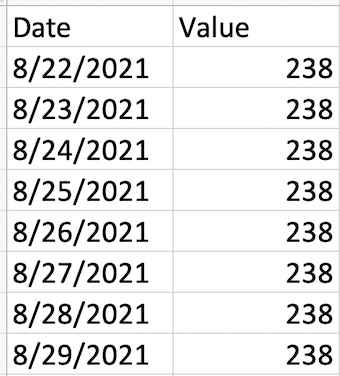
\includegraphics{images/1.11.png}
			\end{figure}
			\item Cho biết số lượng dữ liệu thu thập được theo date và châu lục.
			\begin{figure}[H]
				\centering
				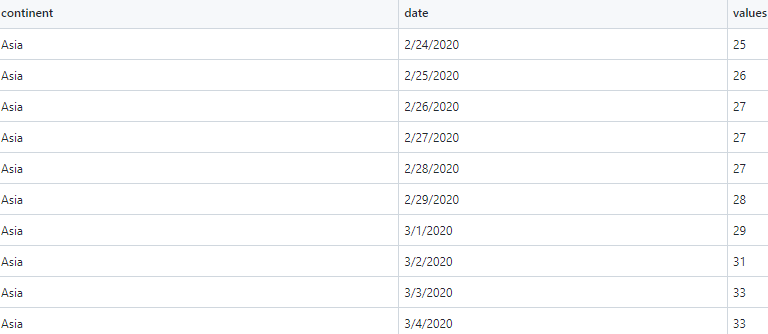
\includegraphics[scale=0.8]{images/1.12.png}
			\end{figure}
            \item Cho biết số lượng dữ liệu thu thập được là lớn nhất theo date và châu lục.
            \begin{figure}[H]
				\centering
				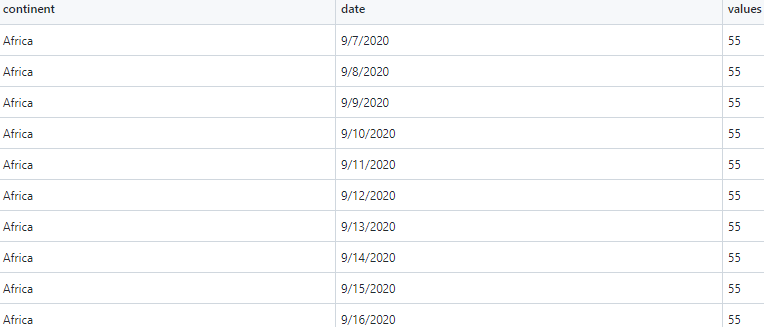
\includegraphics[scale=0.8]{images/1.13.png}
			\end{figure}
            \item Cho biết số lượng dữ liệu thu thập được là nhỏ nhất theo date và châu lục.
            \begin{figure}[H]
				\centering
				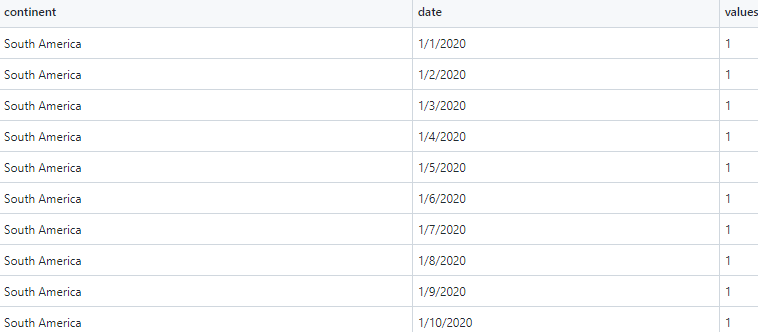
\includegraphics[scale=0.8]{images/1.14.png}
			\end{figure}
            \item Với một date là k và châu lục t cho trước, hãy cho biết số lượng dữ liệu thể hiện thu thập dữ liệu được.
            \begin{figure}[H]
				\centering
				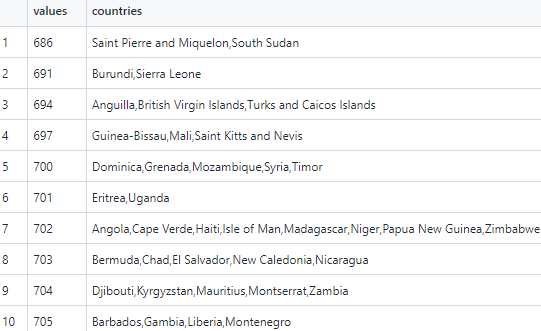
\includegraphics{images/1.15.png}
			\end{figure}
            \item Có đất nước nào mà số lượng dữ liệu thu thập được là bằng nhau không? Hãy cho biết các iso\_code của đất nước đó.
            \begin{figure}[H]
				\centering
				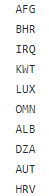
\includegraphics{images/1.16.png}
			\end{figure}
            \item Liệt kê iso\_code, tên đất nước mà chiều dài iso\_code lớn hơn 3.
            \begin{figure}[H]
				\centering
				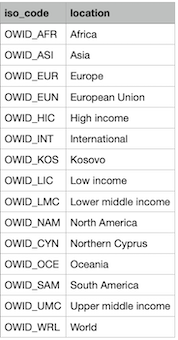
\includegraphics{images/1.17.png}
			\end{figure}
			\end{enumerate}
	\item \textcolor{orange}{Nhóm câu hỏi liên quan đến mô tả thống kê cơ bản dữ liệu}\\
	$\indent$Tứ phân vị là đại lượng mô tả sự phân bố và sự phân tán của tập dữ liệu.
	
    Tứ phân vị có 3 giá trị, đó là tứ phân vị thứ nhất, thứ nhì, và thứ ba.
    
    Ba giá trị này chia một tập hợp dữ liệu (đã sắp xếp dữ liệu theo trật từ từ bé đến lớn) thành 4 phần có số lượng quan sát đều nhau (=1/4 số kết quả quan sát)
    
    Giá trị tứ phân vị thứ hai Q2 chính bằng giá trị trung vị
    
    Giá trị tứ phân vị thứ nhất Q1 bằng trung vị phần dưới
    
    Giá trị tứ phân vị thứ ba Q3 bằng trung vị phần trên
    
    Trong thống kê mô tả, độ lệch chuẩn là thước đo độ phân tán của một tập hợp các giá trị so với giá trị trung bình của chúng. Độ lệch chuẩn của 1 giá trị càng thấp nghĩa là giá trị đó càng gần với giá trị trung bình của tập hợp.
    
    Biểu đồ hộp (Box plot) là biểu đồ diễn tả 5 vị trí phân bố của dữ liệu, đó là: giá trị nhỏ nhất (min), tứ phân vị thứ nhất (Q1), trung vị (median), tứ phân vị thứ 3 (Q3) và giá trị lớn nhất (max).
    
    Các hàm thường sử dụng trong bài ii:
        \begin{itemize}
    \item Hàm names dùng để đặt lại tên cho một đối tượng
    \item Hàm summary cho ta một bảng bao gồm giá trị lớn nhất, nhỏ nhất, tứ phân vị, độ lệch chuẩn, outlier của bảng dữ liệu đầu vào
    \item Hàm rownames và colnames để đặt lại tên cho hàng, cột của bảng dữ liệu
    \item Hàm boxplot để vẽ biểu đồ boxplot
        \end{itemize}
			\begin{enumerate}[1)]
				\item Tính giá trị nhỏ nhất, lớn nhất
				\item Tính tứ phân vị thứ nhất(Q1), thứ hai(Q2), thứ ba(Q3) 
				\item Tính giá trị trung bình (Avg)
				\item Tính giá trị độ lệch chuẩn (Std)
				\item Đếm xem có bao nhiêu outliers, một quan sát mà giá trị của nó nằm trong khoảng sau:\\
				$IQR = Q3 - Q1$\\
				$outliers < Q1 - 1.5*IQR$ hoặc $outliers > Q3 + 1.5*IQR$
				\item Lập bảng mô tả số liệu thống kê cho từng đất nước thuộc về nhóm: \\
				\begin{figure}[H]
					\centering
					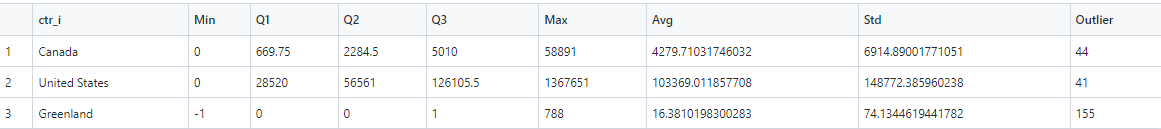
\includegraphics[scale=0.5]{images/2.1.png}
					\vspace{3mm}
					\caption{Số lượng ca nhiễm mới}
					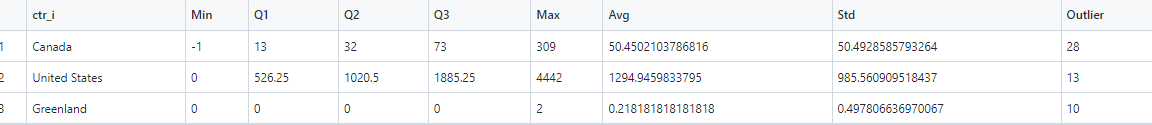
\includegraphics[scale=0.5]{images/2.2.png}
					\vspace{3mm}
					\caption{Số ca tử vong}
				\end{figure}
				\item Vẽ biểu đồ boxplot hay còn được gọi là box-and-whisker cho nhiễm coronavirus
				\begin{figure}[H]
					\centering
					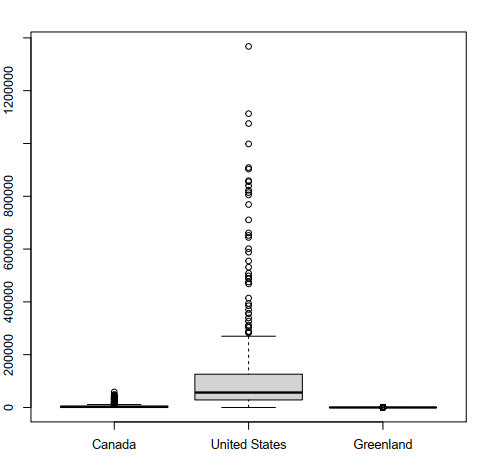
\includegraphics{images/2.3.png}
				\end{figure}
			\end{enumerate}
		\item \textcolor{orange}{Nhóm câu hỏi liên quan đến dữ liệu thể hiện thu thập dữ liệu}\\
	$\indent$Sử dụng hàm p\_load của thư viện Pacman ( đã được tích hợp vào R ở phiên bản 4.1.3) để cài các thư viện chưa có sẵn trong máy vào thêm các thư viện vào chương trình
	
	Các thư viện sử dụng:
	    \begin{itemize}
	\item rio: Nhập xuất file
	\item here: Tạo đường dẫn
	\item tibble: Tạo bảng
        \end{itemize}
        \begin{figure}[H]
            \centering
            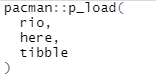
\includegraphics{images/3.0.png}
        \end{figure}
    Nhập file và thiết lập một số giá trị ban đầu
        \begin{itemize}
	\item Sử dụng hàm import kết hợp here để nhập file "owid-covid-data.csv"
	\item Tạo vector “name.country” lưu tên ba nước của nhóm
        \end{itemize}
		\begin{enumerate}[1)]
			\item Có bao nhiêu ngày có số lần dữ liệu không được báo cáo mới.\\
	$\indent$Tạo hàm “ndwithoutrpcases” xử lý yêu cầu đề bài về ca nhiễm khi cung cấp cho hàm tên nước
	    \begin{itemize}
	\item Tạo vector “select” lưu địa chị các dòng chứa tên nước chỉ thị
	\item Sử dụng hàm “subset” với điều kiện là hàm “select” tạo dataframe “covid.data.location” chứa dữ liệu của nước được chọn
	\item Dùng vòng lặp for với số vòng lặp bằng số dòng của của “covid.data.location” đếm số ngày có dữ liệu không được báo cáo mới
	\item Xuất ra giá trị vừa đếm được
	    \begin{figure}[H]
				\centering
				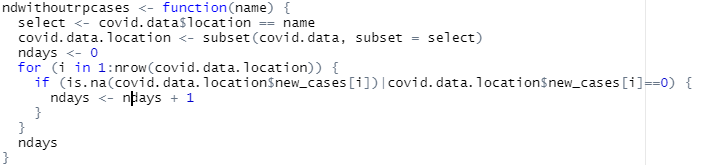
\includegraphics[scale=0.8]{images/3.0.1.png}
		\end{figure}
        \end{itemize}
    $\indent$Sử dụng hàm để tính toán số ngày có dữ liệu ca nhiễm không được báo cáo mới với từng nước, lưu lần lượt giá trị vào 3 biến a, b, c
        \begin{figure}[H]
				\centering
				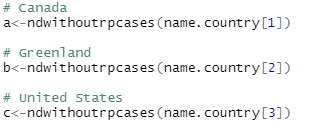
\includegraphics{images/3.0.2.png}
		\end{figure}
	$\indent$Xử lý tương tự với ca tử vong, lưu vào ba biến d, e, f
	
	Tạo dataframe “cau1” lưu các giá trị vừa tạo ở trên
        \begin{figure}[H]
				\centering
				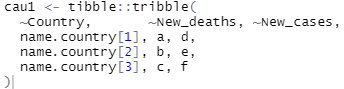
\includegraphics{images/3.0.3.png}
		\end{figure}
			\begin{figure}[H]
				\centering
				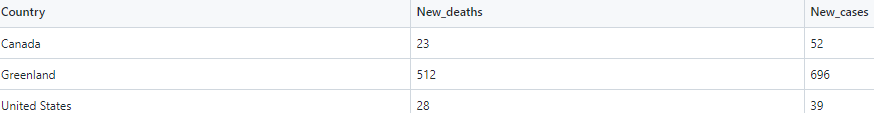
\includegraphics[scale=0.7]{images/3.1.png}
			\end{figure}
			\item Có bao nhiêu ngày có số ca nhiễm/ tử vong là thấp nhất được báo cáo mới.\\
			\begin{itemize}
	\item Tạo hàm “nlowestdayscases” để xử lý yêu cầu đề bài về số ca nhiễm khi được cung cấp tên nước
	\item Tạo dataframe “covid.data.location” chứa dữ liệu từng nước tương tự như câu 1
    \item Tạo biến “ndays” và biến “min” để lưu giá trị thấp nhất, thiết lập giá trị ban đầu cho “ndays” và “min” là 0
	\item Sử dụng vòng lặp for kết hợp câu lệnh if ghép để tìm giá trị đầu tiên khác không phải giá trị rỗng và bằng 0, gán giá trị đó là giá trị min đầu tiên
	\item Dùng vòng lặp for đếm số ngày có số ca nhiễm/tử vong là thấp nhất được báo cáo mới
	\item Xuất ra giá trị vừa tìm được
        \begin{figure}[H]
			\centering
			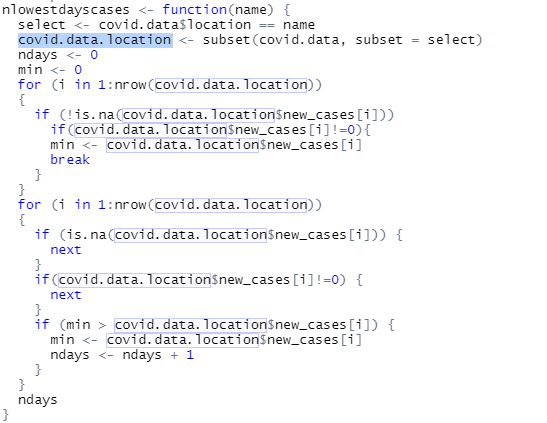
\includegraphics{images/3.0.4.png}
		\end{figure}
	\item Xử lý tương tự ở câu 1, lưu các giá trị lần lượt vào các biến a,b,c,d,e,f sau đó tạo bảng lưu vào dataframe “cau2”
	        \end{itemize}
			\begin{figure}[H]
				\centering
				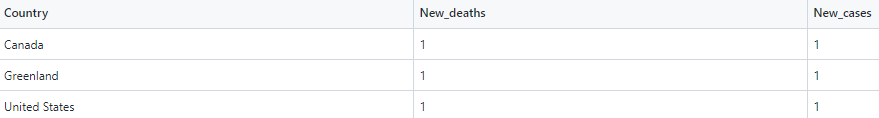
\includegraphics[scale=0.7]{images/3.2.png}
			\end{figure}
			\item Có bao nhiêu ngày có số ca nhiễm/ tử vong là cao nhất được báo cáo mới
			\begin{figure}[H]
				\centering
				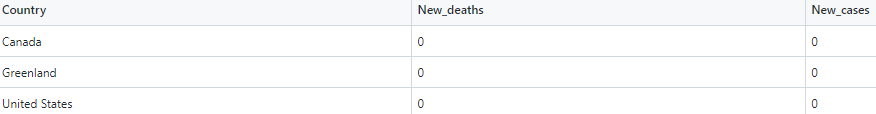
\includegraphics[scale=0.7]{images/3.3.png}
			\end{figure}
			\item Thể hiện bảng số liệu như sau:\\
			Không được báo cáo mới:
			    \begin{itemize}
	\item Sử dụng hàm subset tạo một dataframe lưu giữ liệu của ba nước về tên nước, số ca nhiễm, số ca tử vong và chỉ giữ lại các hàng có số ca nhiễm hoặc ca tử vong bằng 0 hoặc rỗng
	\item Đổi tên 3 cột thành "Countries", "Infections", "Deaths"
	\item Lưu dataframe vừa tạo vào “cau4a”
			    \end{itemize}
			\begin{figure}[H]
				\centering
				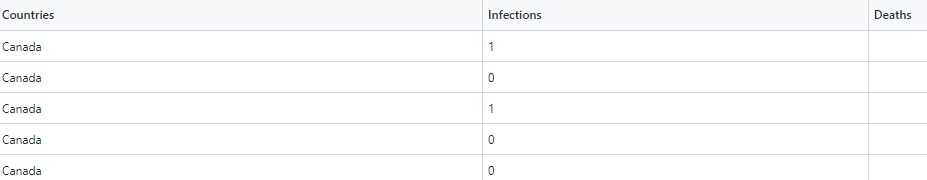
\includegraphics[scale=0.7]{images/3.4.1.png}
			\end{figure}
			Báo cáo mới:
			\begin{figure}[H]
				\centering
				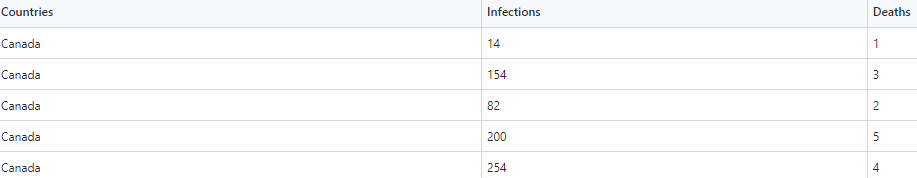
\includegraphics[scale=0.7]{images/3.4.2.png}
			\end{figure}
			\item Cho biết số ngày ngắn nhất liên tiếp mà không có dữ liệu được báo cáo
			    \begin{itemize}
	\item Tạo hàm “short.ds.no.report.cases” để xử lý yêu cầu đề bài về số ca nhiễm khi được cung cấp tên nước
	\item Tạo dataframe “covid.data.location” tương tự các câu trước
	\item Tạo biến “inmissing” để xác định có đang ở trong chuỗi ngày không được báo cáo
	\item Tạo biến “length.of.missing” lưu giá trị của số ngày ngắn nhất liên tiếp mà không có dữ liệu được báo cáo, giá trị ban đầu là toàn bộ số ngày có trong dữ liệu
	\item Tạo biến “temp.length” lưu độ dài chuỗi ngày liên tiếp không được báo cáo vòng lặp for đang chỉ vào
	            \begin{figure}[H]
			    	\centering
			    	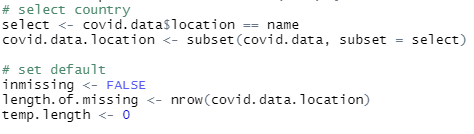
\includegraphics{images/3.0.5.png}
		    	\end{figure}
	\item Nếu dữ liệu không có ngày nào không được báo cáo dữ liệu, length.of.missing =0
	\item Sử dụng vòng lặp for đếm lần lượt chiều dài của các chuỗi số ngày liên tiếp không được báo cáo dữ liệu lưu vào temp.length, nếu temp.length < length.of.missing, gán giá trị của temp.length cho length.of.missing, lần lượt như vậy cho đến hết chương trình
	\item Trả về kết quả vừa tìm được
	\item Lần lượt xử lí cho các nước và lưu vào các biến a,b,c
	\item Tương tự với ca tử vong và lưu vào các biến d, e, f
	\item Tạo bảng chứa các giá trị vừa tìm và lưu vào “cau5”
			    \end{itemize}
			\begin{figure}[H]
				\centering
				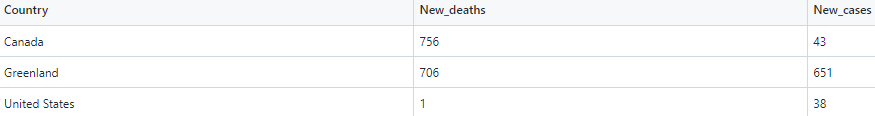
\includegraphics[scale=0.7]{images/3.5.png}
			\end{figure}
			\item Cho biết số ngày dài nhất liên tiếp mà không có dữ liệu được báo cáo
			\begin{figure}[H]
				\centering
				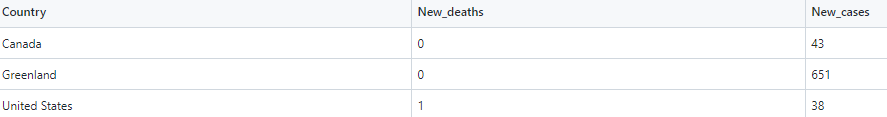
\includegraphics[scale=0.7]{images/3.6.png}
			\end{figure}
			\item Cho biết số ngày ngắn nhất liên tiếp mà không có người nhiễm bệnh mới
			\begin{figure}[H]
				\centering
				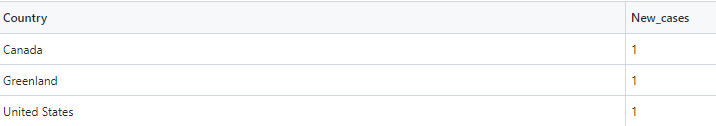
\includegraphics[scale=0.8]{images/3.7.png}
			\end{figure}
			\item Cho biết số ngày dài nhất liên tiếp mà không có người nhiễm bệnh mới
			\begin{figure}[H]
				\centering
				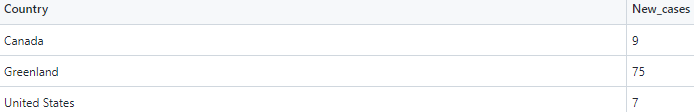
\includegraphics[scale=0.8]{images/3.8.png}
			\end{figure}
		\end{enumerate}
		\item \textcolor{orange}{Nhóm câu hỏi liên quan đến dữ liệu thể hiện thu thập dữ liệu}\\
	$\indent$Biểu đồ tần số tích lũy (cumulative frequency plots) biểu thị những thông tin dạng tích lũy. Nó thể hiện số lượng hay tỉ lệ những quan sát nhỏ hơn hoặc bằng một giá trị cụ thể.
	
    Biểu đồ tần số tương đối thể hiện nội dung y nguyên như biểu đồ tần số tích lũy , chỉ khác một điều đơn vị tính của các cột là tỉ lệ phần trăm.
    
    Biểu đồ phổ là thể hiện sự phân phối về số lượng của một tập dữ liệu.

    Một số thư viện cần dùng: ggplot2, agricolae, ggpubr, lubridate

    Các hàm thường sử dụng trong bài iv:
        \begin{itemize}
\item ggplot để vẽ biểu đồ
\item Hàm ggexport để xuất biểu đồ được vẽ bằng ggplots
\item Hàm strptime chuyển đổi ký tự thành ngày giờ
\item Hàm barplot để vẽ biểu đồ thanh
\item Hàm hist để vẽ biểu đồ tần số
\item Hàm max, min, sum trả về giá trị lớn nhất, nhỏ nhất, tổng của các giá trị nhập vào
        \end{itemize}
		\begin{enumerate}[1]
			\item Vẽ biểu đồ tần số tích lũy quốc gia cho các châu lục
			\begin{figure}[H]
				\centering
				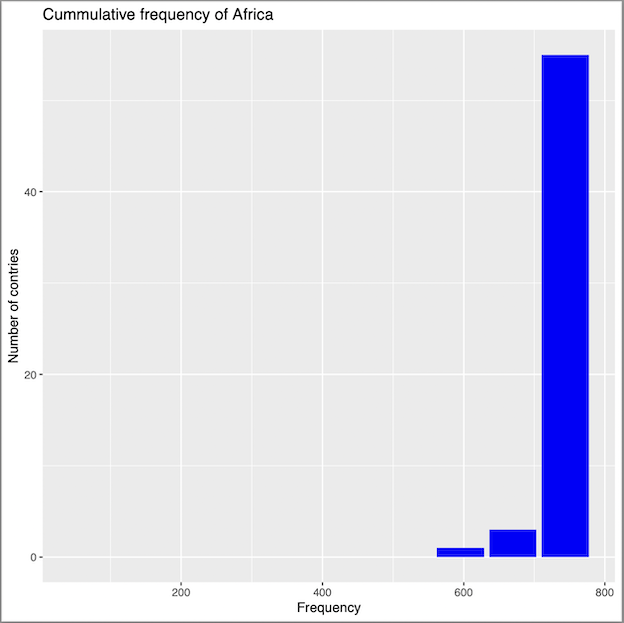
\includegraphics[scale=0.8]{images/4.1.1.png}
				\vspace{5mm}
				\caption{Africa}
			\end{figure}
			\begin{figure}[H]
				\centering
				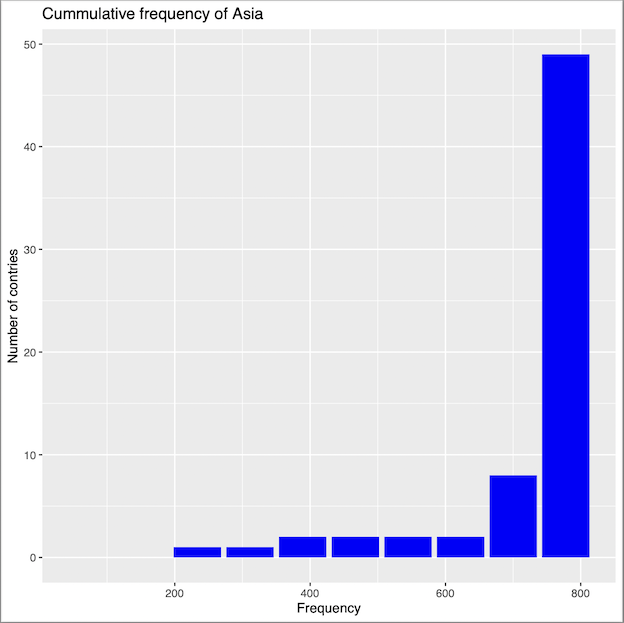
\includegraphics[scale=0.8]{images/4.1.2.png}
				\vspace{5mm}
				\caption{Asia}
			\end{figure}
		\begin{figure}[H]
			\centering
			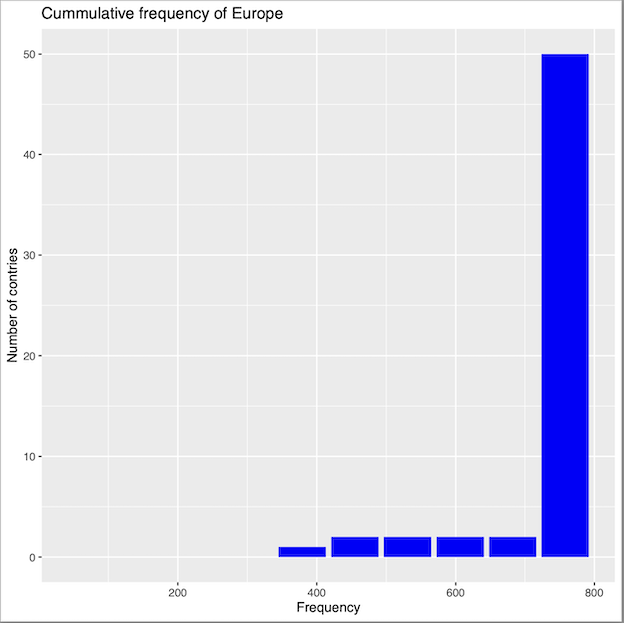
\includegraphics[scale=0.8]{images/4.1.3.png}
			\vspace{5mm}
			\caption{Europe}
		\end{figure}
			\item Vẽ biểu đồ tần số tương đối quốc gia cho các châu lục
			\begin{figure}[H]
				\centering
				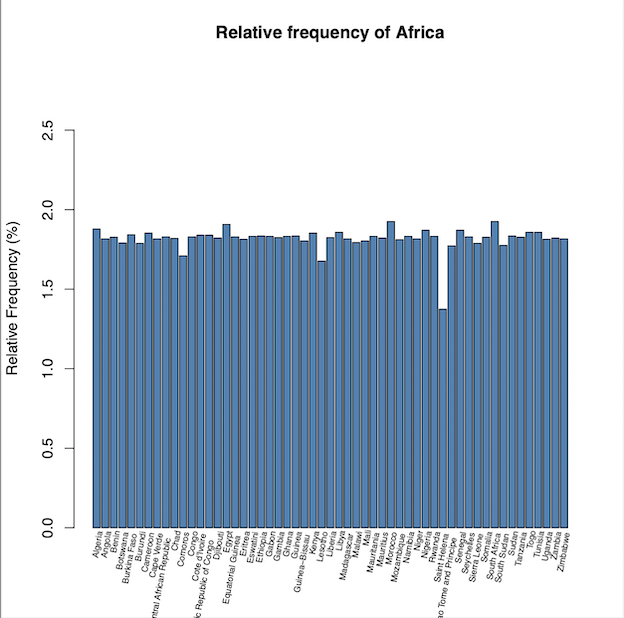
\includegraphics[scale=0.8]{images/4.2.1.png}
			\end{figure}
			\begin{figure}[H]
				\centering
				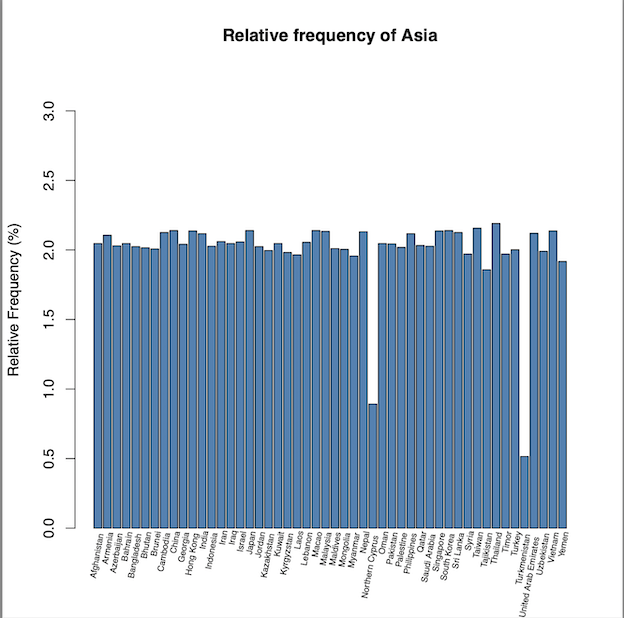
\includegraphics[scale=0.8]{images/4.2.2.png}
			\end{figure}
			\begin{figure}[H]
				\centering
				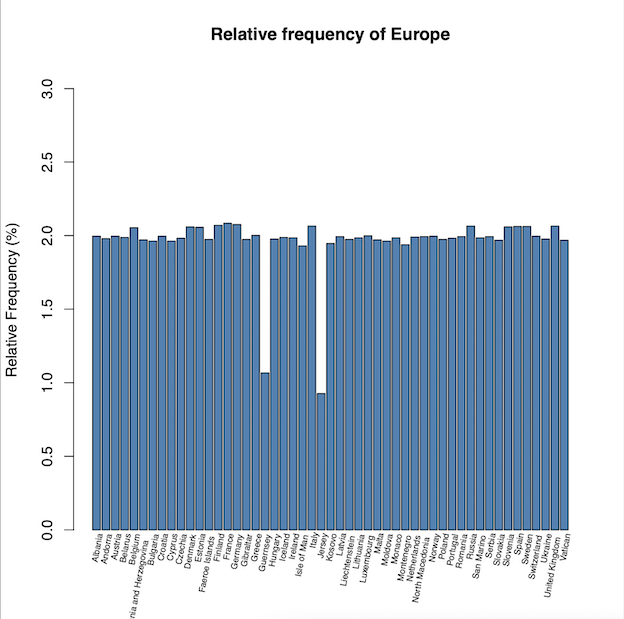
\includegraphics[scale=0.8]{images/4.2.3.png}
			\end{figure}
			\item Vẽ biểu đồ thể hiện nhiễm bệnh đã báo cáo của các quốc gia  mà thuộc về nhóm trong 7 ngày cuối của năm cuối cùng
			\begin{figure}[H]
				\centering
				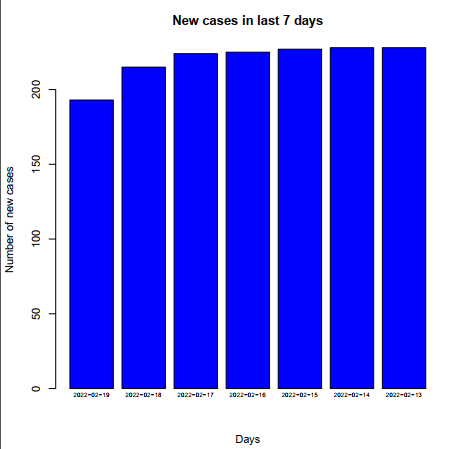
\includegraphics[scale=0.8]{images/4.3.png}
			\end{figure}
			\item Vẽ biểu đồ thể hiện tử vong đã báo cáo của các quốc gia  mà thuộc về nhóm trong 7 ngày cuối của năm cuối cùng
			\begin{figure}[H]
				\centering
				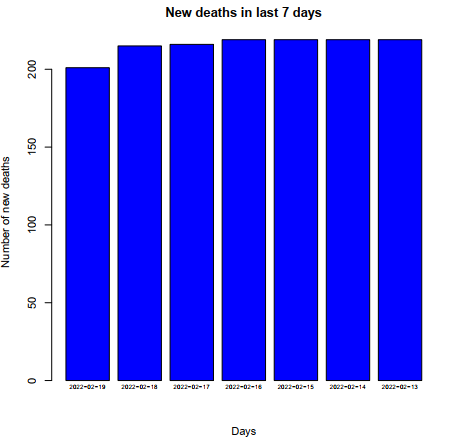
\includegraphics[scale=0.8]{images/4.4.png}
			\end{figure}
			\item Vẽ biểu đồ phổ đất nước xuất hiện outliers cho nhiễm bệnh
			\begin{figure}[H]
				\centering
				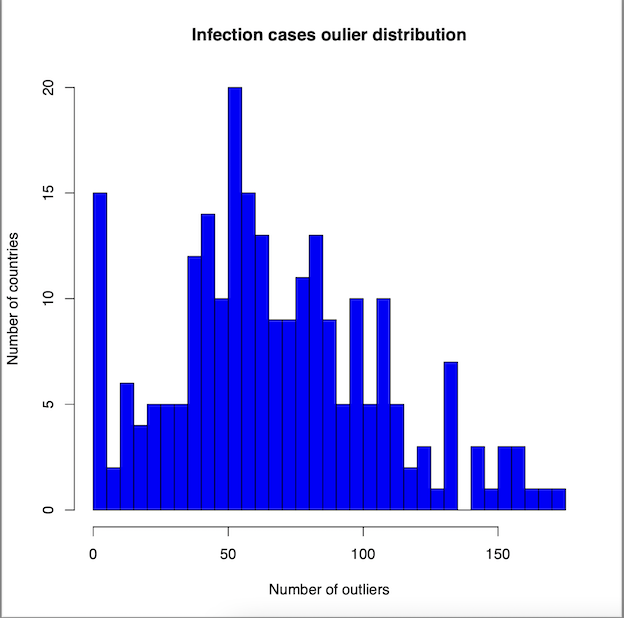
\includegraphics[scale=0.8]{images/4.5.png}
			\end{figure}
			\item Vẽ biểu đồ phổ đất nước xuất hiện outliers cho tử vong
			\begin{figure}[H]
				\centering
				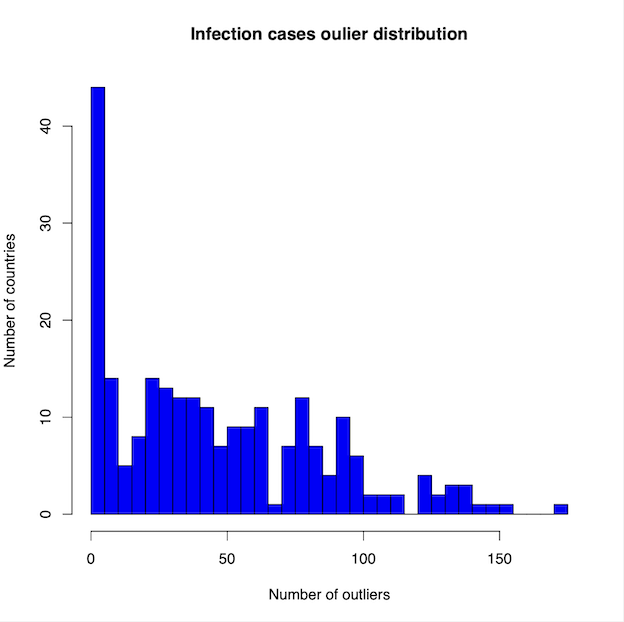
\includegraphics[scale=0.8]{images/4.6.png}
			\end{figure}
		\end{enumerate}
		\item \textcolor{orange}{Nhóm câu hỏi liên quan đến dữ liệu thể hiện thu thập dữ liệu}\\
		$\indent$Với mỗi quốc gia mà thuộc về nhóm, trên từng năm hãy vẽ biểu đồ thể hiện trục Ox là thời gian, trục Oy là nhiễm bệnh/tử vong. Hãy dùng 4 ký số của mã đề để vẽ 4 tháng tương ứng theo ký số đó. Nếu ký số là 0 thì lấy tháng là 10.\\
		Dữ liệu nhiễm bệnh tích lũy cho từng tháng:
		    \begin{itemize}
        \item Số ca nhiễm của 1 ngày trong tháng bằng số ca nhiễm trong ngày hôm đó cộng với tổng số ca nhiễm của tất cả các ngày trước đó.
        \item Lấy số ca nhiễm từng ngày trong tháng chia cho số ca nhiễm của ngày cuối cùng, được phần trăm số ca nhiễm tích lũy mà ngày đó đạt được so với tổng số ca nhiễm trong tháng.
            \end{itemize}
        Tương tự với số ca tử vong.

        Các hàm dùng trong task 5:
            \begin{itemize}
\item Hàm length để lấy độ dài của cột dữ liệu
\item Hàm for và hàm if để cho chạy và lọc dữ liệu cần sử dụng
\item Hàm as.Data để chuyển kiểu dữ liệu sang kiểu "date"
\item Hàm data.frame để nhập hai khung dữ liệu lại thành một
\item Hàm ggplot để vẽ biểu đồ, goemline để vẽ biểu đồ đường, theme để trang trí, labs để đặt tên biểu đồ và trục x, y
\item Hàm is.na để tìm giá trị n/a trong dữ liệu
            \end{itemize}
		    \begin{enumerate}[1]
			\item Biểu đồ thể hiện thu thập dữ liệu nhiễm bệnh cho từng tháng\\
	$\indent$Đầu tiên ta lấy dữ liệu từ file owid-covid-data vào dataRaw và lọc lại các dữ liệu của các nước trong mã đề vào dataMade:
	            \begin{figure}[H]
				    \centering
				    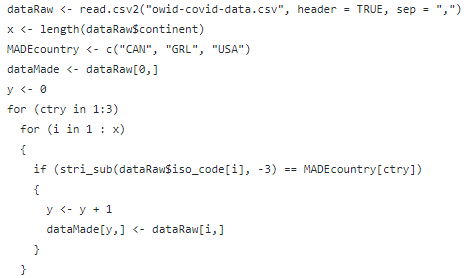
\includegraphics{images/5.0.png}
		    	\end{figure}
	Chuyển kiểu dữ liệu của cột date từ "numberic" sang "date" và đổi tất cả giá trị N/a của cộ new\_deaths và new\_cases thành giá trị 0
	            \begin{figure}[H]
				    \centering
				    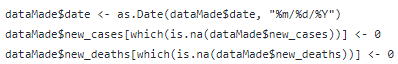
\includegraphics{images/5.0.1.png}
		    	\end{figure}
	Vì 3 câu 1, 2, 3 yêu cầu vẽ biểu đồ trùng khoảng thời gian với nhau nên chỉ cần lọc dữ liệu 1 lần và sử dụng cho cả 3 câu.
	
	VD: Lọc dữ liệu số ca nhiễm bệnh và số ca tử vong ở Canada năm 2020 theo các tháng của mã đề (2, 3, 4, 6) và vẽ biểu đồ số ca nhiễm theo tháng:
	            \begin{figure}[H]
				    \centering
				    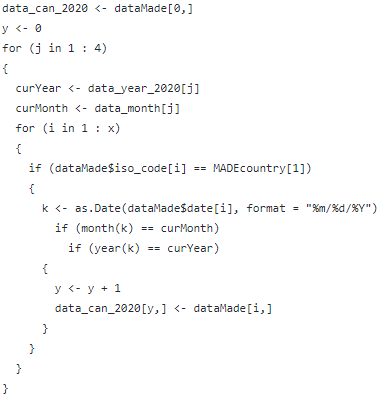
\includegraphics{images/5.0.2.png}
		    	\end{figure}
    Tương tự cho 2 nước Greenland, USA và tương tự trong 2 năm 2021, 2022.
    
    Sau khi có dữ liệu thì dùng ggpplot vẽ biểu đồ:
    
    VD: Biểu đồ số ca nhiễm theo tháng của Canada năm 2020:
                \begin{figure}[H]
				    \centering
				    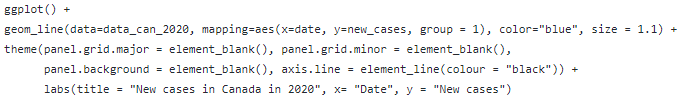
\includegraphics[scale=0.9]{images/5.0.3.png}
		    	\end{figure}
		    	\begin{figure}[H]
				    \centering
				    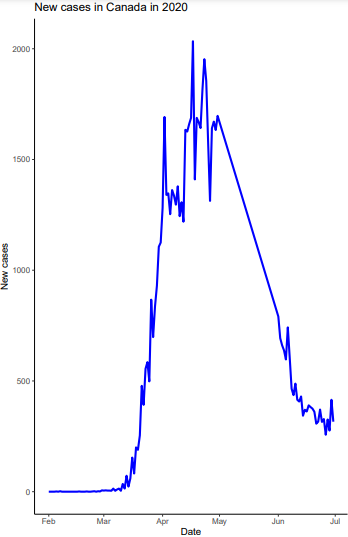
\includegraphics[scale=0.8]{images/5.1.png}
		    	\end{figure}
		    	\begin{figure}[H]
				    \centering
				    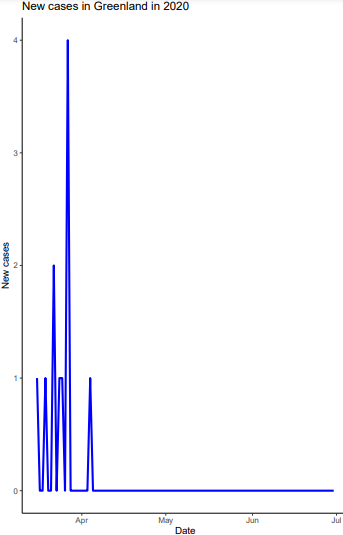
\includegraphics[scale=0.8]{images/5.1.1.png}
		    	\end{figure}
		    	\begin{figure}[H]
				    \centering
				    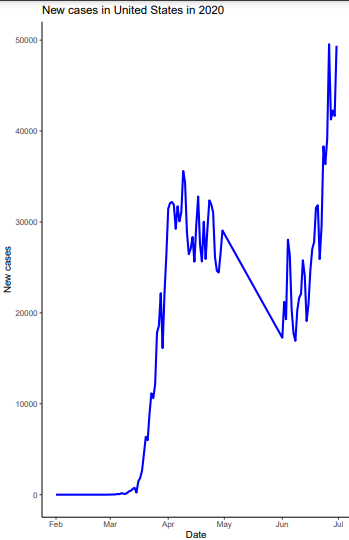
\includegraphics[scale=0.8]{images/5.1.2.png}
		    	\end{figure}
			\item Biểu đồ thể hiện thu thập dữ liệu tử vong cho từng tháng
			\begin{figure}[H]
				\centering
				\includegraphics[scale=0.8]{images/5.2.1.png}
			\end{figure}
			\begin{figure}[H]
				\centering
				\includegraphics[scale=0.8]{images/5.2.2.png}
			\end{figure}
			\begin{figure}[H]
				\centering
				\includegraphics[scale=0.8]{images/5.2.3.png}
			\end{figure}
			\item Biểu đồ thể hiện thu thập dữ liệu gồm nhiễm bệnh và tử vong cho từng tháng 
			\begin{figure}[H]
				\centering
				\includegraphics[scale=0.8]{images/5.3.1.png}
			\end{figure}
			\begin{figure}[H]
				\centering
				\includegraphics[scale=0.8]{images/5.3.2.png}
			\end{figure}
			\begin{figure}[H]
				\centering
				\includegraphics[scale=0.8]{images/5.3.3.png}
			\end{figure}
			\item Biểu đồ thể hiện thu thập dữ liệu nhiễm bệnh gồm 2 tháng cuối của năm
			\begin{figure}[H]
				\centering
				\includegraphics[scale=0.8]{images/5.4.1.png}
			\end{figure}
			\begin{figure}[H]
				\centering
				\includegraphics[scale=0.8]{images/5.4.2.png}
			\end{figure}
			\begin{figure}[H]
				\centering
				\includegraphics[scale=0.8]{images/5.4.3.png}
			\end{figure}
			\item Biểu đồ thể hiện thu thập dữ liệu tử vong gồm 2 tháng cuối của năm
			\begin{figure}[H]
				\centering
				\includegraphics[scale=0.8]{images/5.5.1.png}
			\end{figure}
			\begin{figure}[H]
				\centering
				\includegraphics[scale=0.8]{images/5.5.2.png}
			\end{figure}
			\begin{figure}[H]
				\centering
				\includegraphics[scale=0.8]{images/5.5.3.png}
			\end{figure}
			\item Biểu đồ thể hiện thu thập dữ liệu gồm nhiễm bệnh và tử vong gồm 2 tháng cuối của năm
			\begin{figure}[H]
				\centering
				\includegraphics[scale=0.8]{images/5.6.1.png}
			\end{figure}
			\begin{figure}[H]
				\centering
				\includegraphics[scale=0.8]{images/5.6.2.png}
			\end{figure}
			\begin{figure}[H]
				\centering
				\includegraphics[scale=0.8]{images/5.6.3.png}
			\end{figure}
			\item Biểu đồ thể hiện thu thập dữ liệu nhiễm bệnh tích lũy cho từng tháng\\
	$\indent$Đầu tiên ta tạo 1 vector gồm 4 số để lưu tổng số ca nhiễm của mỗi tháng
	
    VD: Tổng số ca nhiễm mỗi tháng trong năm 2020 của Canada
            \begin{figure}[H]
				\centering
				\includegraphics{images/5.0.4.png}
			\end{figure}
	Tiếp theo, ta biến đổi số ca nhiễm của từng ngày bằng số ca nhiễm của ngày hôm đó cộng với số ca nhiễm của các ngày còn lại trong tháng và lưu vào 1 vector có độ dài bằng độ dài cột new\_cases
	
    VD: Biến đổi số ca nhiễm của Canada trong năm 2020
            \begin{figure}[H]
				\centering
				\includegraphics{images/5.0.5.png}
			\end{figure}
	Biến đổi vector trên thành phần trăm tích lũy số ca nhiễm bằng cách chia cho tổng số ca nhiễm mỗi tháng đã tính
	
    VD: Biến đổi số ca nhiễm của Canada thành phần trăm tích lũy
            \begin{figure}[H]
				\centering
				\includegraphics{images/5.0.6.png}
			\end{figure}
	Cuối cùng, kết hợp vector trên với vector tháng và vẽ biểu đồ 
	
	VD: Biểu đồ phần trăm tích lũy số ca nhiễm bệnh ở Canada theo thời gian là tháng trong năm 2020
	        \begin{figure}[H]
				\centering
				\includegraphics[scale=0.8]{images/5.0.7.png}
			\end{figure}
			\begin{figure}[H]
				\centering
				\includegraphics[scale=0.8]{images/5.7.1.png}
			\end{figure}
			\begin{figure}[H]
				\centering
				\includegraphics[scale=0.8]{images/5.7.2.png}
			\end{figure}
			\begin{figure}[H]
				\centering
				\includegraphics[scale=0.8]{images/5.7.3.png}
			\end{figure}
			\item Biểu đồ thể hiện thu thập dữ liệu tử vong tích lũy cho từng tháng
			\begin{figure}[H]
				\centering
				\includegraphics[scale=0.8]{images/5.8.1.png}
			\end{figure}
			\begin{figure}[H]
				\centering
				\includegraphics[scale=0.8]{images/5.8.2.png}
			\end{figure}
			\begin{figure}[H]
				\centering
				\includegraphics[scale=0.8]{images/5.8.3.png}
			\end{figure}
		\end{enumerate}
		\item \textcolor{orange}{Nhóm câu hỏi liên quan đến dữ liệu thể hiện thu thập dữ liệu}\\
		- Với mỗi quốc gia mà thuộc về nhóm, trên từng năm hãy vẽ biểu đồ thể hiện trục Ox là thời gian, trục Oy là nhiễm bệnh/tử vong. Hãy dùng 4 ký số của mã đề để vẽ 4 tháng tương ứng theo ký số đó. Nếu ký số là 0 thì lấy tháng là 10.
		
		- Dùng trung bình của các ca nhiễm bệnh và tử vong được báo cáo trong 7 ngày gần nhất để loại trừ một số báo cáo không thường xuyên và đưa chúng ta đến gần hơn với con số hàng ngày.
		
		\begin{figure}[H]
		    \centering
			\includegraphics{images/6.0.png}
		\end{figure}
		\begin{figure}[H]
		    \centering
			\includegraphics{images/6.0.1.png}
		\end{figure}
		\begin{figure}[H]
		    \centering
			\includegraphics{images/6.0.2.png}
		\end{figure}
		\begin{figure}[H]
		    \centering
			\includegraphics{images/6.0.3.png}
		\end{figure}
		
		
		\begin{enumerate}[1)]
			\item Biểu đồ thể hiện thu thập dữ liệu nhiễm bệnh cho từng tháng
			\begin{figure}[H]
				\centering
				\includegraphics[scale=0.25]{images/6.1.1.png}
			\end{figure}
			\begin{figure}[H]
				\centering
				\includegraphics[scale=0.25]{images/6.1.2.png}
			\end{figure}
			\begin{figure}[H]
				\centering
				\includegraphics[scale=0.25]{images/6.1.3.png}
			\end{figure}
			\item Biểu đồ thể hiện thu thập dữ liệu tử vong cho từng tháng
			\begin{figure}[H]
				\centering
				\includegraphics[scale=0.25]{images/6.2.1.png}
			\end{figure}
			\begin{figure}[H]
				\centering
				\includegraphics[scale=0.25]{images/6.2.2.png}
			\end{figure}
			\begin{figure}[H]
				\centering
				\includegraphics[scale=0.25]{images/6.2.3.png}
			\end{figure}
			\item Biểu đồ thể hiện thu thập dữ liệu gồm nhiễm bệnh và tử vong cho từng tháng
			\begin{figure}[H]
				\centering
				\includegraphics[scale=0.25]{images/6.3.1.png}
			\end{figure}
			\begin{figure}[H]
				\centering
				\includegraphics[scale=0.25]{images/6.3.2.png}
			\end{figure}
			\begin{figure}[H]
				\centering
				\includegraphics[scale=0.25]{images/6.3.3.png}
			\end{figure}
			\item Biểu đồ thể hiện thu thập dữ liệu nhiễm bệnh gồm 2 tháng cuối của năm
			\begin{figure}[H]
				\centering
				\includegraphics[scale=0.25]{images/6.4.1.png}
			\end{figure}
			\begin{figure}[H]
				\centering
				\includegraphics[scale=0.25]{images/6.4.2.png}
			\end{figure}
			\begin{figure}[H]
				\centering
				\includegraphics[scale=0.25]{images/6.4.3.png}
			\end{figure}
			\item Biểu đồ thể hiện thu thập dữ liệu tử vong gồm 2 tháng cuối của năm
			\begin{figure}[H]
				\centering
				\includegraphics[scale=0.25]{images/6.5.1.png}
			\end{figure}
			\begin{figure}[H]
				\centering
				\includegraphics[scale=0.25]{images/6.5.2.png}
			\end{figure}
			\begin{figure}[H]
				\centering
				\includegraphics[scale=0.25]{images/6.5.3.png}
			\end{figure}
			\item Biểu đồ thể hiện thu thập dữ liệu gồm nhiễm bệnh và tử vong gồm 2 tháng cuối của năm
			\begin{figure}[H]
				\centering
				\includegraphics[scale=0.25]{images/6.6.1.png}
			\end{figure}
			\begin{figure}[H]
				\centering
				\includegraphics[scale=0.25]{images/6.6.2.png}
			\end{figure}
			\begin{figure}[H]
				\centering
				\includegraphics[scale=0.25]{images/6.6.3.png}
			\end{figure}
			\item Biểu đồ thể hiện thu thập dữ liệu nhiễm bệnh tích lũy cho từng tháng
			\begin{figure}[H]
				\centering
				\includegraphics[scale=0.25]{images/6.7.1.png}
			\end{figure}
			\begin{figure}[H]
				\centering
				\includegraphics[scale=0.25]{images/6.7.2.png}
			\end{figure}
			\begin{figure}[H]
				\centering
				\includegraphics[scale=0.25]{images/6.7.3.png}
			\end{figure}
			\item Biểu đồ thể hiện thu thập dữ liệu tử vong tích lũy cho từng tháng
			\begin{figure}[H]
				\centering
				\includegraphics[scale=0.25]{images/6.8.1.png}
			\end{figure}
			\begin{figure}[H]
				\centering
				\includegraphics[scale=0.25]{images/6.8.2.png}
			\end{figure}
			\begin{figure}[H]
				\centering
				\includegraphics[scale=0.25]{images/6.8.3.png}
			\end{figure}
		\end{enumerate}
		\item \textcolor{orange}{Nhóm câu hỏi liên quan đến dữ liệu thể hiện thu thập dữ liệu}\\
		- Trên từng năm hãy vẽ biểu đồ thể hiện trục Ox là thời gian, trục Oy là nhiễm bệnh/tử vong. Hãy dùng 4 ký số của mã đề để vẽ 4 tháng tương ứng theo ký số đó. Nếu ký số là 0 thì lấy tháng là 10.\\
		
		Đầu tiên ta lấy dữ liệu từ file owid-covid-data vào dataRaw và lọc lại các dữ liệu của tất cả 18 quốc gia trong đề vào dataMade:
        \begin{figure}[H]
			\centering
			\includegraphics{images/7.0.png}
		\end{figure}
		
		\begin{enumerate}[1]
			\item Biểu đồ thể hiện thu thập dữ liệu nhiễm bệnh theo thời gian là tháng của tất cả quốc gia\\
			Tạo các vector ngày tháng cần thiết để lọc dữ liệu theo thời gian là tháng
			\begin{figure}[H]
				\centering
				\includegraphics{images/7.0.1.png}
			\end{figure}
			Tạo 1 vector có chiều dài là 162 để lưu dữ liệu nhiễm bệnh theo từng tháng của tất cả các quốc gia
			\begin{figure}[H]
				\centering
				\includegraphics{images/7.0.2.png}
			\end{figure}
			Chạy vòng lặp với điều kiện để lưu dữ liệu cần thiết vào vector newcases
			\begin{figure}[H]
				\centering
				\includegraphics{images/7.0.3.png}
			\end{figure}
			Kết hợp vector trên với vector tháng năm tạo thành bảng dữ liệu nhiễm bệnh theo thời gian là tháng của tất cả các nước
			\begin{figure}[H]
				\centering
				\includegraphics{images/7.0.4.png}
			\end{figure}
			Vẽ biểu đồ thể hiện thu thập dữ liệu nhiễm bệnh cho từng tháng dựa vào bảng trên
			\begin{figure}[H]
				\centering
				\includegraphics{images/7.0.5.png}
			\end{figure}
			\begin{figure}[H]
				\centering
				\includegraphics[scale=0.2]{images/7.1.png}
			\end{figure}
			\item Biểu đồ thể hiện thu thập dữ liệu tử vong theo thời gian là tháng của tất cả quốc gia
			\begin{figure}[H]
				\centering
				\includegraphics[scale=0.2]{images/7.2.png}
			\end{figure}
			\item Biểu đồ thể hiện thu thập dữ liệu nhiễm bệnh theo thời gian là 2 tháng cuối của năm của tất cả quốc gia
			\begin{figure}[H]
				\centering
				\includegraphics[scale=0.2]{images/7.3.png}
			\end{figure}
			\item Biểu đồ thể hiện thu thập dữ liệu tử vong theo thời gian là 2 tháng cuối của năm của tất cả quốc gia
			\begin{figure}[H]
				\centering
				\includegraphics[scale=0.2]{images/7.4.png}
			\end{figure}
			\item Biểu đồ thể hiện thu thập dữ liệu nhiễm bệnh tương đối tích lũy theo thời gian là 2 tháng cuối của năm của tất cả quốc gia\\
			Đầu tiên, tạo và lưu dữ liệu tích lũy nhiễm bệnh theo ngày trong 2 tháng cuối năm vào vector có độ dài 61
			\begin{figure}[H]
				\centering
				\includegraphics[scale=0.8]{images/7.0.6.png}
			\end{figure}
			Tiếp theo, tạo vector có độ dài tương ứng để lưu dữ liệu nhiễm bệnh tương đối tích lũy theo thời gian là tháng bằng cách chia tất cả giá trị cho giá trị cuối cùng
			\begin{figure}[H]
				\centering
				\includegraphics[scale=0.8]{images/7.0.7.png}
			\end{figure}
			Cuối cùng, tạo bảng dữ liệu và vẽ biểu đồ
			\begin{figure}[H]
				\centering
				\includegraphics[scale=0.7]{images/7.0.8.png}
			\end{figure}
			Năm 2021 làm tương tự
			\begin{figure}[H]
				\centering
				\includegraphics[scale=0.2]{images/7.5.1.png}
			\end{figure}
			\begin{figure}[H]
				\centering
				\includegraphics[scale=0.2]{images/7.5.2.png}
			\end{figure}
			\item Biểu đồ thể hiện thu thập dữ liệu tử vong tương đối tích lũy theo thời gian là 2 tháng cuối của năm của tất cả quốc gia
			\begin{figure}[H]
				\centering
				\includegraphics[scale=0.2]{images/7.6.1.png}
			\end{figure}
			\begin{figure}[H]
				\centering
				\includegraphics[scale=0.2]{images/7.6.2.png}
			\end{figure}
		\end{enumerate}
		\item \textcolor{orange}{Nhóm câu hỏi liên quan đến dữ liệu thể hiện thu thập dữ liệu}\\
		Trên từng năm hãy vẽ biểu đồ thể hiện trục Ox là thời gian, trục Oy là nhiễm bệnh/tử vong. Hãy dùng 4 ký số của mã đề để vẽ 4 tháng tương ứng theo ký số đó. Nếu ký số là 0 thì lấy tháng là 10.\\
		\begin{center}
		****CƠ SỞ LÝ THUYẾT****\\
		\end{center}
		
        -Nghiên cứu tình trạng nhiễm bệnh và tử vong tích lũy theo thời gian là tháng tất cả các quốc gia vào tháng 2,3,4,6.\\

        -Sử dụng ngôn ngữ lập trình R để chọn lọc dữ liệu\\

        -Lọc và xử lý dữ liệu có isocode là "OWID\_WRL", ta được các thông tin cần thiết về số ca tử vong do COVID-19 trên thế giới.\\

        -Sử dụng ngôn ngữ lập trình R để tính toán:\\

        -Bảng giá trị trung bình 7 ngày gần nhất (TB) của một dãy số A được tính như sau:\\
        \begin{itemize}
            \item TB[1]: nhận A[1]\\
            \item TB[2]: lấy giá trị trung bình của A[1], A[2]\\
            \item TB[3]: lấy giá trị trung bình của A[1],A[2],A[3]\\
            \item .\\
            \item .\\
            \item .\\
            \item TB[7]: lấy giá trị trung bình của A[1], A[2], ..., A[7]\\
            \item TB[i] (i>7): lấy giá trị trung bình của A[i-6], A[i-5],..., A[i]\\
        \end{itemize}

        -Từng bước khởi gán các giá trị tổng số ca nhiễm, tử vong theo tháng, sau đó tính trung bình 7 ngày gần nhất của từng ngày và đồng thời tạo bảng giá trị theo từng tháng, từng năm và từng nhóm câu hỏi của đề bài\\

        -Sử dụng các lệnh của ngôn ngữ R để vẽ biểu đồ cho từng nhóm câu hỏi\\

        -Đầu tiên, tạo các biến cần thiết\\
        ggplot(NULL,aes(<các ngày>,<số ca mới>)): khởi tạo hệ trục Oxy với các miền giá trị tương ứng Ox,Oy\\
        geomline(data=<new>,col="<colour>"): vẽ đường biểu diễn các ca mới (new) trong tháng, có màu là (colour)\\
        labs(title="<tên biểu đồ>",x="<tên trục Ox>,y="<tên trục Oy>"): thêm nhãn cho biểu đồ\\
        
        -Tiếp theo, kết hợp các biến vào một để tạo biểu đồ\\
        graphcases<tháng hiện tại><-ggplot()+geomline()+labs(): tạo biểu đồ theo tháng đang tính toán( 4 tháng tất cả)\\
        
        -Cuối cùng, lưu các biểu đồ vừa tạo vào một file lưu trữ\\
        -Ví dụ:\\
        \begin{itemize}
            \item ggsave(filename="task8subtask1case2020.pdf",\\
            \item plot=ggarrange(graphcasesthangHai, graphcasesthangBa,graphcasesthangTu,graphcasesthangSau, nrow=4, ncol=1, common.legend=TRUE),\\
            \item scale=1,\\
            \item width=10,\\
            \item height=25,\\
            \item units=c("in"),\\
            \item dpi=300)\\
        \end{itemize}
        --->tạo file có tên "task8subtask1case2020.pdf" lưu số ca mới trong năm 2020 theo yêu cầu tiểu câu hỏi 1 với 4 biểu đồ riêng biệt của 4 tháng 2,3,4,6 xếp dọc 4 hàng 1 cột, tỉ lệ phóng đại 1.0, chiều rộng 10 inch, chiều cao 25 inch\\
        
        (Có sử dụng thêm các lệnh trên biểu đồ để trang trí, hiệu chỉnh)
		\begin{enumerate}[1)]
			\item Biểu đồ thể hiện thu thập dữ liệu nhiễm bệnh theo thời gian là tháng của tất cả quốc gia theo trung bình 7 ngày gần nhất
			\begin{figure}[H]
				\centering
				\includegraphics[height=23cm,width=13cm]{images/8.1.1.png}
			\end{figure}
			\begin{figure}[H]
				\centering
				\includegraphics[height=23cm,width=13cm]{images/8.1.2.png}
			\end{figure}
			\begin{figure}[H]
				\centering
				\includegraphics[scale=0.2]{images/8.1.3.png}
			\end{figure}
			\item Biểu đồ thể hiện thu thập dữ liệu tử vong theo thời gian là tháng của tất cả quốc gia theo trung bình 7 ngày gần nhất
			\begin{figure}[H]
				\centering
				\includegraphics[height=23cm,width=13cm]{images/8.2.1.png}
			\end{figure}
			\begin{figure}[H]
				\centering
				\includegraphics[height=23cm,width=13cm]{images/8.2.2.png}
			\end{figure}
			\begin{figure}[H]
				\centering
				\includegraphics[scale=0.2]{images/8.2.3.png}
			\end{figure}
			\item Biểu đồ thể hiện thu thập dữ liệu nhiễm bệnh theo thời gian là 2 tháng của năm của tất cả quốc giaị theo trung bình 7 ngày gần nhất
			\begin{figure}[H]
				\centering
				\includegraphics[height=23cm,width=13cm]{images/8.3.1.png}
			\end{figure}
			\begin{figure}[H]
				\centering
				\includegraphics[height=23cm,width=13cm]{images/8.3.2.png}
			\end{figure}
			\begin{figure}[H]
				\centering
				\includegraphics[scale=0.2]{images/8.3.3.png}
			\end{figure}
			\item Biểu đồ thể hiện thu thập dữ liệu tử vong theo thời gian là 2 tháng của năm của tất cả quốc gia theo trung bình 7 ngày gần nhất
			\begin{figure}[H]
				\centering
				\includegraphics[height=23cm,width=13cm]{images/8.4.1.png}
			\end{figure}
			\begin{figure}[H]
				\centering
				\includegraphics[height=23cm,width=13cm]{images/8.4.2.png}
			\end{figure}
			\begin{figure}[H]
				\centering
				\includegraphics[scale=0.2]{images/8.4.3.png}
			\end{figure}
			\item Biểu đồ thể hiện thu thập dữ liệu nhiễm bệnh tích lũy theo thời gian là 2 tháng của năm của tất cả quốc giaị theo trung bình 7 ngày gần nhất
			\begin{figure}[H]
				\centering
				\includegraphics[height=23cm,width=13cm]{images/8.5.1.png}
			\end{figure}
			\begin{figure}[H]
				\centering
				\includegraphics[height=23cm,width=13cm]{images/8.5.2.png}
			\end{figure}
			\begin{figure}[H]
				\centering
				\includegraphics[scale=0.2]{images/8.5.3.png}
			\end{figure}
			\item Biểu đồ thể hiện thu thập dữ liệu tử vong tích lũy theo thời gian là 2 tháng của năm của tất cả quốc gia theo trung bình 7 ngày gần nhất
			\begin{figure}[H]
				\centering
				\includegraphics[height=23cm,width=13cm]{images/8.6.1.png}
			\end{figure}
			\begin{figure}[H]
				\centering
				\includegraphics[height=23cm,width=13cm]{images/8.6.2.png}
			\end{figure}
			\begin{figure}[H]
				\centering
				\includegraphics[scale=0.2]{images/8.6.3.png}
			\end{figure}
		\end{enumerate}
		\item \textcolor{orange}{Nhóm câu hỏi liên quan đến dữ liệu thể hiện thu thập dữ liệu}\\
		\begin{center}
		    ****CƠ SỞ LÝ THUYẾT****\\
		\end{center}
		-----Correlation Coefficient là gì?-----\\
		
		\begin{itemize}
		    \item Hệ số tương quan là một thước đo thống kê về độ mạnh yếu của mối quan hệ giữa các chuyển động tương đối của hai biến, các giá trị này nằm trong khoảng từ -1,0 đến 1,0. Một số được tính toán lớn hơn 1,0 hoặc nhỏ hơn -1,0 có nghĩa là đã xảy ra lỗi trong phép đo tương quan. Tương quan -1,0 cho thấy mối tương quan âm tuyệt đối, trong khi mức tương quan 1,0 cho thấy mối tương quan dương tuyệt đối. Tương quan 0,0 cho thấy không có mối quan hệ tuyến tính giữa chuyển động của hai biến.\\
		
		    \item Có một loại hệ số tương quan, nhưng phổ biến nhất là hệ số tương quan Pearson (R), hệ số này chỉ ra độ mạnh và hướng của mối quan hệ tuyến tính giữa hai biến. Đây cũng là hệ số sẽ được sử dụng để tính toán trong phần trình bày này.\\
		
		    \item Giá trị chính xác bằng 1,0 nghĩa là có một mối quan hệ dương tuyệt đối giữa hai biến. Đối với một biến số tăng dương thì biến số thứ hai cũng tăng dương.Giá trị chính xác bằng -1,0 nghĩa là có một mối quan hệ âm tuyệt đối giữa hai biến. Điểu này cho thấy các biến chuyển động ngược chiểu nhau. Đối với một biến số tăng dương thì biến số thứ hai sẽ giảm xuống. Nếu mối tương quan giữa hai biến là 0 thì không có mối quan hệ tuyến tính giữa chúng.\\
		
		    \item Độ mạnh của mối quan hệ thay đổi theo mức độ dựa trên giá trị của hệ số tương quan. Ví dụ, giá trị 0,2 cho thấy có mối tương quan dương giữa hai biến. Các nhà phân tích trong một số lĩnh vực nghiên cứu không coi các mối tương quan là quan trọng cho đến khi giá trị vượt qua ít nhất 0,8. Tuy nhiên, hệ số tương quan có giá trị tuyệt đối từ 0,9 trở lên sẽ thể hiện một mối quan hệ rất chặt chẽ.\\
		 \end{itemize}
		
		- Trong bài báo cáo này, một mối quan hệ giữa hai biến được coi là:\\
		\begin{itemize}
	    \item Mạnh (Strong) nếu trị tuyệt đối hệ số tương quan giữa chúng lớn hơn 0,7,\\
		\item Trung bình (Moderate) nếu trị tuyệt đối hệ số tương quan giữa chúng lớn hơn 0,5 và bé hơn bằng 0,7,\\
		\item Yếu (Weak) nếu trị tuyệt đối hệ số tương quan giữa chúng lớn hơn 0,3 và bé hơn bằng 0,5,\\
		\item Rất yếu(Very Weak) nếu trị tuyệt đối hệ số tương quan giữa chúng bé hơn bằng 0,3.\\
    	\end{itemize}
		
		- Nghiên cứu tình trạng nhiễm bệnh và tử vong tích lũy theo thời gian là tháng của 3 nước theo MADE vào 4 tháng 2,3,4,6\\
		
		- Lọc và xử lý dữ liệu có isocode là CAN,GRL,USA ta được các thông tin cần thiết về số ca mắc mới và số ca tử vong do COVID19 tại các nước Canada, Greenland và Hoa Kỳ.\\
		
		- Sử dụng ngôn ngữ lập trình R để tính toán:\\
		Từng bước khởi gán các giá trị tống số ca nhiễm, ca tử vong theo tháng sau đó tính tổng  tích lũy từng ngày, đông thời lập bảng tỉ lệ phần trăm trên tổng số ca.\\
		Sử dụng hàm cor(x,y,"pearson") để tính Pearson coefficient correlation giữa 2 biến, sau đó kết hợp kết quả với nhận xét về độ mạnh của mối tương quan đưa vào biểu đồ của subtask1\\
		
		- Sử dụng các lệnh của ngôn ngữ R để vẽ biểu đồ:\\
		- Đầu tiên, tạo các biến cần thiết\\
		+ ggplot(NULL,aes(<các ngày>, <số ca mới>)): khởi tạo hệ trục Oxy với các miền giá trị tương ứng Ox,Oy\\
		+ geomarea(data=<new>, col="<colour>"): vẽ miền biểu diễn các ca mới (new) trong tháng, có màu là (colour)\\
		+ labs(title="<tên biểu đồ>",x="<tên trục Ox>",y="<tên trục Oy>"): thêm nhãn cho biểu đồ\\
		+annotate(geom="<kiểu chú thích>",x=<tọa độ x>, y=<tọa độ y>,...): thêm chú thích cho biểu đồ\\
		
		- Tiếp theo, kết hợp các biến vào một để tạo biểu đồ\\
		graphcases<tháng hiện tại><-ggplot()+geomarea()+labs()+annotate(): tạo biểu đồ theo tháng đang tính toán (4 tháng tất cả)\\
		
		- Cuối cùng, lưu các biểu đồ vừa tạo vào một file lưu trữ\\
		Ví dụ:\\
		\begin{itemize}
	    \item ggsave(filename="task9subtask1Canadanews2020.pdf",\\
		\item plot=ggarrange(graphcasesthangHai, graphcasesthangBa,graphcasesthangTu,graphcasesthangSau, nrow=4, ncol=1, common.legend=TRUE),\\
        \item scale=1,\\
        \item width=10,\\
        \item height=25,\\
        \item units=c("in"),\\
        \item dpi=300)\\
	    \end{itemize}
         --->tạo file có tên "task9subtask1Canadanews2020.pdf" lưu số ca mới trong năm 2020 theo yêu cầu tiểu câu hỏi 1 với 4 biểu đồ riêng biệt của 4 tháng 2,3,4,6 xếp dọc 4 hàng 1 cột, tỉ lệ phóng đại 1.0, chiều rộng 10 inch, chiều cao 25 inch\\
        
        (Có sử dụng thêm các lệnh trên biểu đồ để trang trí, hiệu chỉnh)
        
		

		\begin{enumerate}[1)]
			\item Vẽ biểu đồ thể hiện phần trăm giữa nhiễm bệnh tích lũy trên tổng nhiễm bệnh và phần trăm tử vong tích lũy trên tổng số tử vong cho từng quốc gia theo thời gian. Vẽ 2 đường trên cùng biểu đồ\\
			
			Trên từng quốc gia riêng của nhóm hãy vẽ biểu đồ thể hiện trục Ox là nhiễm bệnh, trục Oy là tử vong. Hãy lấy 4 tháng theo 4 ký số mã đề thể hiện. Nếu ký số là 0 thì lấy tháng là 10.
			\item Xét tương quan trong mỗi tháng, 
			\item Xét tương quan trong mỗi tháng theo trung bình 7 ngày gần nhất\\
			\begin{center}
			    ------KẾT QUẢ CHO BÀI IX:------
			\end{center}
			\begin{figure}[H]
				\centering
				\includegraphics[height=23cm,width=13cm]{images/9.1.png}
			\end{figure}
			\begin{figure}[H]
				\centering
				\includegraphics[height=23cm,width=13cm]{images/9.2.png}
			\end{figure}
			\begin{figure}[H]
				\centering
				\includegraphics[height=23cm,width=13cm]{images/9.3.png}
			\end{figure}
			\begin{figure}[H]
				\centering
				\includegraphics[height=23cm,width=13cm]{images/9.4.png}
			\end{figure}
			\begin{figure}[H]
				\centering
				\includegraphics[height=23cm,width=13cm]{images/9.5.png}
			\end{figure}
			\begin{figure}[H]
				\centering
				\includegraphics[height=23cm,width=13cm]{images/9.6.png}
			\end{figure}
		\end{enumerate}
		\item \textcolor{orange}{Nhóm câu hỏi riêng}\\
        2) So sánh tình trạng tử vong của các quốc gia trong 7 ngày cuối của năm cuối cùng\\
        \begin{figure}[H]
            \centering
            \includegraphics[scale=0.5]{images/10.2.png}
        \end{figure}
        * Nhận xét:\\
        -  Trong 7 ngày cuối trong số liệu của năm cuối cùng (từ 13/02 -19/02 năm 2022):\\
        \begin{itemize}
            \item Greenland khá may mắn vì gần như không có một ca tử vong nào, cho thấy nước này đảm bảo được sự an toàn trước đại dịch.\\
            \item Bên cạnh đó, Canada lại có số người chết mỗi ngày còn khá nhiều (dao động trong vài chục ca).\\
            \item Tuy vậy, người dân Hoa Kỳ vẫn chịu nhiều sự đau thương nhất, khi mà có đến 5 trên 7 ngày số người chết lên tới 4 chữ số.\\
        \end{itemize}
        ->Những điều này chứng tỏ những ảnh hưởng nặng nề mà đại dịch này để lại cho con người, những con virut mang lại hậu quả sức khỏe hết sức nguy hiểm không thể chủ quan.\\
        4) Với k là mốc bùng phát dịch, hãy xác định k và cho biết các khoảng thời gian bùng phát\\
        Cơ sở lý thuyết về bùng phát bệnh dịch:\\
        - Lấy k làm mốc để xác định khoảng thời gian bùng phát.\\
        - Với k là khi số ca nhiễm bệnh tăng đột biến trên khoảng 200 phần trăm so với 20 ngày trước, số ca nhiễm bệnh phải lớn hơn 50000 thì ta sẽ coi đó là lúc bùng phát bệnh dịch.\\
        - Từ đó, ta sử dụng ngôn ngữ lập trình R để chỉ ra các thời điểm bắt đầu bùng phát.
        \begin{figure}[H]
            \centering
            \includegraphics{images/10.4.png}
        \end{figure}
        6) Khoảng thời gian bùng phát nhiễm bệnh lớn nhất giữa các quốc gia có chồng lên nhau không, Cho biết khoảng thời gian giao nhau đó?\\
        - Các mốc bùng phát bệnh dịch của các quốc gia là:\\
        \begin{itemize}
            \item CANADA\\
            \item 2021-12-20\\
            \item GREENLAND\\
            \item NULL\\
            \item USA\\
            \item 2021-12-28\\
        \end{itemize}
        - Dễ dàng nhận thấy 2 nước Canada và Hoa Kỳ có cùng khoảng thời gian bắt đầu bùng phát bệnh dịch vào cuối năm ngoái (2021)\\
        - Đây cũng là thời điểm 2 nước này có kì nghỉ lễ đặc biệt nhất trong năm (Lễ Giáng Sinh và chuẩn bị qua năm mới).\\
        - Do đó, từ tháng 12 năm 2021 đến tháng 1 năm 2022, số ca nhiễm bệnh đã tăng không kiểm soát, với số ca nhiễm cao nhất trong 1 ngày đã tăng gấp 10 lần so với trước khi dịch bệnh bùng nổ.
\end{enumerate}
	\section{Tổng kết}\label{end}
	$\indent$Phân tích dữ liệu về dịch bệnh Covid có ý nghĩa quan trọng trong việc đánh giá mức độ nghiêm trọng của đại dịch trên toàn thế giới. Ngoài ra, những dữ liệu riêng của từng châu lục, hay từng quốc gia giúp ta dễ dàng xác định được những khu vực có dịch bệnh bùng nổ, hay những nơi có dấu hiệu xuất hiện của dịch bệnh để tìm ra những biện pháp xử lý, phòng tránh phù hợp. Những kết quả ta phân tích được trong quá khứ có ý nghĩa thực tế trong việc dự đoán những con số sẽ xuất hiện trong tương lai. Qua bài tập lớn này, ngoài việc tiếp xúc và rèn luyện với ngôn ngữ mới là R và Latex, ta còn được nâng cao kỹ năng phân tích số liệu cũng như biểu diễn các số liệu thống kê một cách dễ hiểu cho người xem.
	%%%%%%%%%%%%%%%%%%%%
	\addcontentsline{toc}{section}{Tài liệu}
	\begin{thebibliography}{99999}
		\bibitem[Dal]{Dal}{Dalgaard, P.} {\em Introductory Statistics with R.}  Springer 2008.
		
		\bibitem[K-Z]{K-Z}{Kenett, R. S. and Zacks, S.}
		{\em Modern Industrial Statistics: with applications in R, MINITAB and JMP,} 2nd ed.,  John Wiley and Sons, 2014.
		
		\bibitem[Ker]{Ker}{Kerns, G. J.}
		{\em Introduction to Probability and Statistics Using R,} 2nd ed., CRC 2015.
		
	\end{thebibliography}
\end{document}